% Options for packages loaded elsewhere
\PassOptionsToPackage{unicode}{hyperref}
\PassOptionsToPackage{hyphens}{url}
\PassOptionsToPackage{dvipsnames,svgnames,x11names}{xcolor}
%
\documentclass[
]{article}
\usepackage{amsmath,amssymb}
\usepackage{iftex}
\ifPDFTeX
  \usepackage[T1]{fontenc}
  \usepackage[utf8]{inputenc}
  \usepackage{textcomp} % provide euro and other symbols
\else % if luatex or xetex
  \usepackage{unicode-math} % this also loads fontspec
  \defaultfontfeatures{Scale=MatchLowercase}
  \defaultfontfeatures[\rmfamily]{Ligatures=TeX,Scale=1}
\fi
\usepackage{lmodern}
\ifPDFTeX\else
  % xetex/luatex font selection
\fi
% Use upquote if available, for straight quotes in verbatim environments
\IfFileExists{upquote.sty}{\usepackage{upquote}}{}
\IfFileExists{microtype.sty}{% use microtype if available
  \usepackage[]{microtype}
  \UseMicrotypeSet[protrusion]{basicmath} % disable protrusion for tt fonts
}{}
\makeatletter
\@ifundefined{KOMAClassName}{% if non-KOMA class
  \IfFileExists{parskip.sty}{%
    \usepackage{parskip}
  }{% else
    \setlength{\parindent}{0pt}
    \setlength{\parskip}{6pt plus 2pt minus 1pt}}
}{% if KOMA class
  \KOMAoptions{parskip=half}}
\makeatother
\usepackage{xcolor}
\usepackage[margin=1in]{geometry}
\usepackage{color}
\usepackage{fancyvrb}
\newcommand{\VerbBar}{|}
\newcommand{\VERB}{\Verb[commandchars=\\\{\}]}
\DefineVerbatimEnvironment{Highlighting}{Verbatim}{commandchars=\\\{\}}
% Add ',fontsize=\small' for more characters per line
\usepackage{framed}
\definecolor{shadecolor}{RGB}{248,248,248}
\newenvironment{Shaded}{\begin{snugshade}}{\end{snugshade}}
\newcommand{\AlertTok}[1]{\textcolor[rgb]{0.94,0.16,0.16}{#1}}
\newcommand{\AnnotationTok}[1]{\textcolor[rgb]{0.56,0.35,0.01}{\textbf{\textit{#1}}}}
\newcommand{\AttributeTok}[1]{\textcolor[rgb]{0.13,0.29,0.53}{#1}}
\newcommand{\BaseNTok}[1]{\textcolor[rgb]{0.00,0.00,0.81}{#1}}
\newcommand{\BuiltInTok}[1]{#1}
\newcommand{\CharTok}[1]{\textcolor[rgb]{0.31,0.60,0.02}{#1}}
\newcommand{\CommentTok}[1]{\textcolor[rgb]{0.56,0.35,0.01}{\textit{#1}}}
\newcommand{\CommentVarTok}[1]{\textcolor[rgb]{0.56,0.35,0.01}{\textbf{\textit{#1}}}}
\newcommand{\ConstantTok}[1]{\textcolor[rgb]{0.56,0.35,0.01}{#1}}
\newcommand{\ControlFlowTok}[1]{\textcolor[rgb]{0.13,0.29,0.53}{\textbf{#1}}}
\newcommand{\DataTypeTok}[1]{\textcolor[rgb]{0.13,0.29,0.53}{#1}}
\newcommand{\DecValTok}[1]{\textcolor[rgb]{0.00,0.00,0.81}{#1}}
\newcommand{\DocumentationTok}[1]{\textcolor[rgb]{0.56,0.35,0.01}{\textbf{\textit{#1}}}}
\newcommand{\ErrorTok}[1]{\textcolor[rgb]{0.64,0.00,0.00}{\textbf{#1}}}
\newcommand{\ExtensionTok}[1]{#1}
\newcommand{\FloatTok}[1]{\textcolor[rgb]{0.00,0.00,0.81}{#1}}
\newcommand{\FunctionTok}[1]{\textcolor[rgb]{0.13,0.29,0.53}{\textbf{#1}}}
\newcommand{\ImportTok}[1]{#1}
\newcommand{\InformationTok}[1]{\textcolor[rgb]{0.56,0.35,0.01}{\textbf{\textit{#1}}}}
\newcommand{\KeywordTok}[1]{\textcolor[rgb]{0.13,0.29,0.53}{\textbf{#1}}}
\newcommand{\NormalTok}[1]{#1}
\newcommand{\OperatorTok}[1]{\textcolor[rgb]{0.81,0.36,0.00}{\textbf{#1}}}
\newcommand{\OtherTok}[1]{\textcolor[rgb]{0.56,0.35,0.01}{#1}}
\newcommand{\PreprocessorTok}[1]{\textcolor[rgb]{0.56,0.35,0.01}{\textit{#1}}}
\newcommand{\RegionMarkerTok}[1]{#1}
\newcommand{\SpecialCharTok}[1]{\textcolor[rgb]{0.81,0.36,0.00}{\textbf{#1}}}
\newcommand{\SpecialStringTok}[1]{\textcolor[rgb]{0.31,0.60,0.02}{#1}}
\newcommand{\StringTok}[1]{\textcolor[rgb]{0.31,0.60,0.02}{#1}}
\newcommand{\VariableTok}[1]{\textcolor[rgb]{0.00,0.00,0.00}{#1}}
\newcommand{\VerbatimStringTok}[1]{\textcolor[rgb]{0.31,0.60,0.02}{#1}}
\newcommand{\WarningTok}[1]{\textcolor[rgb]{0.56,0.35,0.01}{\textbf{\textit{#1}}}}
\usepackage{graphicx}
\makeatletter
\def\maxwidth{\ifdim\Gin@nat@width>\linewidth\linewidth\else\Gin@nat@width\fi}
\def\maxheight{\ifdim\Gin@nat@height>\textheight\textheight\else\Gin@nat@height\fi}
\makeatother
% Scale images if necessary, so that they will not overflow the page
% margins by default, and it is still possible to overwrite the defaults
% using explicit options in \includegraphics[width, height, ...]{}
\setkeys{Gin}{width=\maxwidth,height=\maxheight,keepaspectratio}
% Set default figure placement to htbp
\makeatletter
\def\fps@figure{htbp}
\makeatother
\setlength{\emergencystretch}{3em} % prevent overfull lines
\providecommand{\tightlist}{%
  \setlength{\itemsep}{0pt}\setlength{\parskip}{0pt}}
\setcounter{secnumdepth}{5}
\usepackage[french]{babel}
\ifLuaTeX
  \usepackage{selnolig}  % disable illegal ligatures
\fi
\usepackage{bookmark}
\IfFileExists{xurl.sty}{\usepackage{xurl}}{} % add URL line breaks if available
\urlstyle{same}
\hypersetup{
  pdfauthor={Manal Derghal, Khalil Ounis, Taqwa Ben Romdhane},
  colorlinks=true,
  linkcolor={Maroon},
  filecolor={Maroon},
  citecolor={Blue},
  urlcolor={blue},
  pdfcreator={LaTeX via pandoc}}

\title{Analyse des algorithmes de Maximum Subarray 1D\\
\strut ~M2 Data Science Algorithmique}
\author{Manal Derghal, Khalil Ounis, Taqwa Ben Romdhane}
\date{Lundi 7 avril 2025}

\begin{document}
\maketitle

{
\hypersetup{linkcolor=}
\setcounter{tocdepth}{2}
\tableofcontents
}
\noindent\hrulefill

\section{Description du problème et
objectif}\label{description-du-probluxe8me-et-objectif}

Le problème du Maximum Subarray 1D consiste à trouver la sous-séquence
contiguë d'un tableau numérique dont la somme des éléments est maximale.
Ce problème classique en algorithmique a des applications en analyse de
données financières, bioinformatique et traitement du signal.

\href{https://en.wikipedia.org/wiki/Maximum_subarray_problem}{La page
Wikipedia du Maximum Subarray} présente plusieurs approches
algorithmiques pour résoudre ce problème. Nous nous concentrons sur deux
méthodes :

\begin{enumerate}
\def\labelenumi{\arabic{enumi}.}
\tightlist
\item
  Algorithme naïf : complexité O(n²)
\item
  Algorithme de Kadane : complexité optimale O(n)
\end{enumerate}

Nos objectifs sont :\\
a. d'implémenter ces algorithmes en R et C++ et évaluer le gain de
temps.\\
b. de confirmer les complexités théoriques par des simulations
intensives.

\begin{center}\rule{0.5\linewidth}{0.5pt}\end{center}

\section{Un premier exemple}\label{un-premier-exemple}

Le package se télécharge ainsi :

\begin{Shaded}
\begin{Highlighting}[]
\NormalTok{devtools}\SpecialCharTok{::}\FunctionTok{install\_github}\NormalTok{(}\StringTok{"AMATERASU11/MaximumSubarray"}\NormalTok{)}
\end{Highlighting}
\end{Shaded}

et ses fonctions sont rendues disponibles sur Rstudio ainsi :

\begin{Shaded}
\begin{Highlighting}[]
\FunctionTok{library}\NormalTok{(MaximumSubarray)}
\end{Highlighting}
\end{Shaded}

On simule un petit exemple d'un vecteur \texttt{v} de taille
\texttt{100}

\begin{Shaded}
\begin{Highlighting}[]
\FunctionTok{set.seed}\NormalTok{(}\DecValTok{123}\NormalTok{)}
\NormalTok{v }\OtherTok{\textless{}{-}} \FunctionTok{sample}\NormalTok{(}\SpecialCharTok{{-}}\DecValTok{100}\SpecialCharTok{:}\DecValTok{100}\NormalTok{, }\DecValTok{100}\NormalTok{, }\AttributeTok{replace =} \ConstantTok{TRUE}\NormalTok{)}
\end{Highlighting}
\end{Shaded}

On teste les 4 algorithmes implémentés avec des noms explicites :

\begin{itemize}
\tightlist
\item
  \texttt{max\_subarray\_sum\_naive}
\item
  \texttt{max\_subarray\_sum\_opt}
\item
  \texttt{max\_subarray\_sum\_naive\_Rcpp}
\item
  \texttt{max\_subarray\_sum\_opt\_Rcpp}
\end{itemize}

Cela donne :

\begin{Shaded}
\begin{Highlighting}[]
\NormalTok{v}
\end{Highlighting}
\end{Shaded}

\begin{verbatim}
##   [1]  58  78 -87  94  69 -51  17 -58 -87  17  52 -11 -10  96 -10  84  -9  36
##  [19]  -2 -29 -75 -94  69  36  63 -23 -20 -58   2  16 -25  42 -69   8 -94  36
##  [37]  68 -27 -78  54  87 -48  34 -48  54  65 -67 -32 -29 -25 -38  40  -4 -10
##  [55]  52 -63 -80 -60  74 -11 -41 -85  15  -7 -95  99 -15 -15 -62  58  17 -51
##  [73] -67 -97 -88 -32  26  52 -49 -79 -12  59 -76 -66  67  11 -71  39  58  20
##  [91]   9  57 -37  41  98 -34  50  21 -22 -16
\end{verbatim}

\begin{Shaded}
\begin{Highlighting}[]
\FunctionTok{max\_subarray\_sum\_naive}\NormalTok{(v)}
\end{Highlighting}
\end{Shaded}

\begin{verbatim}
## $sum
## [1] 329
## 
## $subarray
##  [1]  67  11 -71  39  58  20   9  57 -37  41  98 -34  50  21
\end{verbatim}

\begin{Shaded}
\begin{Highlighting}[]
\FunctionTok{max\_subarray\_sum\_naive\_Rcpp}\NormalTok{(v)}
\end{Highlighting}
\end{Shaded}

\begin{verbatim}
## $sum
## [1] 329
## 
## $subarray
##  [1]  67  11 -71  39  58  20   9  57 -37  41  98 -34  50  21
\end{verbatim}

\begin{Shaded}
\begin{Highlighting}[]
\FunctionTok{max\_subarray\_sum\_opt}\NormalTok{(v)}
\end{Highlighting}
\end{Shaded}

\begin{verbatim}
## $sum
## [1] 329
## 
## $subarray
##  [1]  67  11 -71  39  58  20   9  57 -37  41  98 -34  50  21
\end{verbatim}

\begin{Shaded}
\begin{Highlighting}[]
\FunctionTok{max\_subarray\_sum\_opt\_Rcpp}\NormalTok{(v)}
\end{Highlighting}
\end{Shaded}

\begin{verbatim}
## $sum
## [1] 329
## 
## $subarray
##  [1]  67  11 -71  39  58  20   9  57 -37  41  98 -34  50  21
\end{verbatim}

\begin{center}\rule{0.5\linewidth}{0.5pt}\end{center}

\section{Comparaison R avec C++}\label{comparaison-r-avec-c}

On va faire des comparaisons pour les deux types d'algorithme en R et
C++ pour quantifier leur différence de performance.

La fonction \texttt{one.simu.time} retourne le temps recherché, et
\texttt{one.simu} sera utilisé par \texttt{microbenchmark}, on retourne
le temps en ms

\begin{Shaded}
\begin{Highlighting}[]
\FunctionTok{library}\NormalTok{(microbenchmark)}

\NormalTok{one.simu.time }\OtherTok{\textless{}{-}} \ControlFlowTok{function}\NormalTok{(n, func) \{}
  
\NormalTok{  v }\OtherTok{\textless{}{-}} \FunctionTok{sample}\NormalTok{(}\SpecialCharTok{{-}}\DecValTok{100}\SpecialCharTok{:}\DecValTok{100}\NormalTok{, n, }\AttributeTok{replace =} \ConstantTok{TRUE}\NormalTok{)}

  \ControlFlowTok{if}\NormalTok{ (func }\SpecialCharTok{==} \StringTok{"Naive1D"}\NormalTok{) \{}
\NormalTok{    t }\OtherTok{\textless{}{-}} \FunctionTok{microbenchmark}\NormalTok{(}\FunctionTok{max\_subarray\_sum\_naive}\NormalTok{(v), }\AttributeTok{times =} \DecValTok{1}\NormalTok{)}\SpecialCharTok{$}\NormalTok{time }\SpecialCharTok{/} \FloatTok{1e6}
\NormalTok{  \} }\ControlFlowTok{else} \ControlFlowTok{if}\NormalTok{ (func }\SpecialCharTok{==} \StringTok{"Naive1D\_cpp"}\NormalTok{) \{}
\NormalTok{    t }\OtherTok{\textless{}{-}} \FunctionTok{microbenchmark}\NormalTok{(}\FunctionTok{max\_subarray\_sum\_naive\_Rcpp}\NormalTok{(v), }\AttributeTok{times =} \DecValTok{1}\NormalTok{)}\SpecialCharTok{$}\NormalTok{time }\SpecialCharTok{/} \FloatTok{1e6}
\NormalTok{  \} }\ControlFlowTok{else} \ControlFlowTok{if}\NormalTok{ (func }\SpecialCharTok{==} \StringTok{"Kadane1D"}\NormalTok{) \{}
\NormalTok{    t }\OtherTok{\textless{}{-}} \FunctionTok{microbenchmark}\NormalTok{(}\FunctionTok{max\_subarray\_sum\_opt}\NormalTok{(v), }\AttributeTok{times =} \DecValTok{1}\NormalTok{)}\SpecialCharTok{$}\NormalTok{time }\SpecialCharTok{/} \FloatTok{1e6}
\NormalTok{  \} }\ControlFlowTok{else} \ControlFlowTok{if}\NormalTok{ (func }\SpecialCharTok{==} \StringTok{"Kadane1D\_cpp"}\NormalTok{) \{}
\NormalTok{    t }\OtherTok{\textless{}{-}} \FunctionTok{microbenchmark}\NormalTok{(}\FunctionTok{max\_subarray\_sum\_opt\_Rcpp}\NormalTok{(v), }\AttributeTok{times =} \DecValTok{1}\NormalTok{)}\SpecialCharTok{$}\NormalTok{time }\SpecialCharTok{/} \FloatTok{1e6}
\NormalTok{  \} }\ControlFlowTok{else}\NormalTok{ \{}
    \FunctionTok{stop}\NormalTok{(}\StringTok{"fonction inconnue"}\NormalTok{)}
\NormalTok{  \}}

  \FunctionTok{return}\NormalTok{(}\FunctionTok{round}\NormalTok{(t, }\DecValTok{2}\NormalTok{))}
\NormalTok{\}}
\end{Highlighting}
\end{Shaded}

\subsection{Un essai}\label{un-essai}

\subsubsection{Temps d'exécution en R}\label{temps-dexuxe9cution-en-r}

Sur un exemple, on obtient :

\begin{Shaded}
\begin{Highlighting}[]
\CommentTok{\# Simulation sur une matrice de taille n}
\NormalTok{n }\OtherTok{\textless{}{-}} \DecValTok{10000}

\CommentTok{\# Exécuter la simulation}
\NormalTok{res\_naive }\OtherTok{\textless{}{-}} \FunctionTok{one.simu.time}\NormalTok{(n,}\StringTok{"Naive1D"}\NormalTok{)}
\NormalTok{res\_kadane }\OtherTok{\textless{}{-}} \FunctionTok{one.simu.time}\NormalTok{(n, }\StringTok{"Kadane1D"}\NormalTok{)}

\CommentTok{\# Afficher les résultats}
\FunctionTok{cat}\NormalTok{(}\StringTok{"time\_naive:"}\NormalTok{, res\_naive,}\StringTok{"ms}\SpecialCharTok{\textbackslash{}n}\StringTok{"}\NormalTok{)}
\end{Highlighting}
\end{Shaded}

\begin{verbatim}
## time_naive: 2717.72 ms
\end{verbatim}

\begin{Shaded}
\begin{Highlighting}[]
\FunctionTok{cat}\NormalTok{(}\StringTok{"time\_kadane:"}\NormalTok{, res\_kadane, }\StringTok{"ms"}\NormalTok{)}
\end{Highlighting}
\end{Shaded}

\begin{verbatim}
## time_kadane: 0.95 ms
\end{verbatim}

\subsubsection{Temps d'exécution en C++}\label{temps-dexuxe9cution-en-c}

sur un vecteur de taille 10000 on obtient les résultats suivants :

\begin{Shaded}
\begin{Highlighting}[]
\CommentTok{\# Simulation sur une matrice de taille n}
\NormalTok{n }\OtherTok{\textless{}{-}} \DecValTok{10000}

\NormalTok{res\_naive\_cpp }\OtherTok{\textless{}{-}} \FunctionTok{one.simu.time}\NormalTok{(n,}\StringTok{"Naive1D\_cpp"}\NormalTok{)}
\NormalTok{res\_Kadane\_cpp }\OtherTok{\textless{}{-}} \FunctionTok{one.simu.time}\NormalTok{(n,}\StringTok{"Kadane1D\_cpp"}\NormalTok{)}

\CommentTok{\# Afficher les résultats}
\FunctionTok{cat}\NormalTok{(}\StringTok{"time\_naive\_cpp:"}\NormalTok{ ,res\_naive\_cpp,}\StringTok{"ms}\SpecialCharTok{\textbackslash{}n}\StringTok{"}\NormalTok{)}
\end{Highlighting}
\end{Shaded}

\begin{verbatim}
## time_naive_cpp: 26.93 ms
\end{verbatim}

\begin{Shaded}
\begin{Highlighting}[]
\FunctionTok{cat}\NormalTok{(}\StringTok{"time\_kadane\_cpp:"}\NormalTok{,res\_Kadane\_cpp, }\StringTok{"ms"}\NormalTok{)}
\end{Highlighting}
\end{Shaded}

\begin{verbatim}
## time_kadane_cpp: 0.1 ms
\end{verbatim}

\subsection{Simulations avec
répétitions}\label{simulations-avec-ruxe9puxe9titions}

On reproduit ces comparaisons de manière plus robuste:

\begin{Shaded}
\begin{Highlighting}[]
\NormalTok{nbSimus }\OtherTok{\textless{}{-}} \DecValTok{10}

\NormalTok{time\_naive }\OtherTok{\textless{}{-}} \FunctionTok{rep}\NormalTok{(}\DecValTok{0}\NormalTok{, nbSimus); time\_naive\_cpp }\OtherTok{\textless{}{-}} \FunctionTok{rep}\NormalTok{(}\DecValTok{0}\NormalTok{, nbSimus);}
\NormalTok{time\_kadane }\OtherTok{\textless{}{-}} \FunctionTok{rep}\NormalTok{(}\DecValTok{0}\NormalTok{, nbSimus); time\_kadane\_cpp }\OtherTok{\textless{}{-}} \FunctionTok{rep}\NormalTok{(}\DecValTok{0}\NormalTok{, nbSimus)}

\ControlFlowTok{for}\NormalTok{(i }\ControlFlowTok{in} \DecValTok{1}\SpecialCharTok{:}\NormalTok{nbSimus)\{time\_naive[i] }\OtherTok{\textless{}{-}} \FunctionTok{one.simu.time}\NormalTok{(n, }\AttributeTok{func =} \StringTok{"Naive1D"}\NormalTok{)\}}
\ControlFlowTok{for}\NormalTok{(i }\ControlFlowTok{in} \DecValTok{1}\SpecialCharTok{:}\NormalTok{nbSimus)\{time\_naive\_cpp[i] }\OtherTok{\textless{}{-}} \FunctionTok{one.simu.time}\NormalTok{(n, }\AttributeTok{func =} \StringTok{"Naive1D\_cpp"}\NormalTok{)\}}
\ControlFlowTok{for}\NormalTok{(i }\ControlFlowTok{in} \DecValTok{1}\SpecialCharTok{:}\NormalTok{nbSimus)\{time\_kadane[i] }\OtherTok{\textless{}{-}} \FunctionTok{one.simu.time}\NormalTok{(n, }\AttributeTok{func =} \StringTok{"Kadane1D"}\NormalTok{)\}}
\ControlFlowTok{for}\NormalTok{(i }\ControlFlowTok{in} \DecValTok{1}\SpecialCharTok{:}\NormalTok{nbSimus)\{time\_kadane\_cpp[i] }\OtherTok{\textless{}{-}} \FunctionTok{one.simu.time}\NormalTok{(n, }\AttributeTok{func =} \StringTok{"Kadane1D\_cpp"}\NormalTok{)\}}
\end{Highlighting}
\end{Shaded}

\subsubsection{Gain R versus C++}\label{gain-r-versus-c}

\begin{Shaded}
\begin{Highlighting}[]
\NormalTok{naive\_speedup\_cpp }\OtherTok{\textless{}{-}} \FunctionTok{mean}\NormalTok{(time\_naive) }\SpecialCharTok{/} \FunctionTok{mean}\NormalTok{(time\_naive\_cpp)}
\NormalTok{kadane\_speedup\_cpp }\OtherTok{\textless{}{-}} \FunctionTok{mean}\NormalTok{(time\_kadane) }\SpecialCharTok{/} \FunctionTok{mean}\NormalTok{(time\_kadane\_cpp)}
\FunctionTok{cat}\NormalTok{(}\StringTok{"le gain R vs cpp pour naif:"}\NormalTok{, }\FunctionTok{round}\NormalTok{(naive\_speedup\_cpp,}\DecValTok{2}\NormalTok{),}\StringTok{"ms}\SpecialCharTok{\textbackslash{}n}\StringTok{"}\NormalTok{)}
\end{Highlighting}
\end{Shaded}

\begin{verbatim}
## le gain R vs cpp pour naif: 81.66 ms
\end{verbatim}

\begin{Shaded}
\begin{Highlighting}[]
\FunctionTok{cat}\NormalTok{(}\StringTok{"le gain R vs cpp pour Kadane:"}\NormalTok{, }\FunctionTok{round}\NormalTok{(kadane\_speedup\_cpp,}\DecValTok{2}\NormalTok{),}\StringTok{"ms}\SpecialCharTok{\textbackslash{}n}\StringTok{"}\NormalTok{)}
\end{Highlighting}
\end{Shaded}

\begin{verbatim}
## le gain R vs cpp pour Kadane: 9.4 ms
\end{verbatim}

\subsubsection{Gain Naif Versus Kadane en R et
C++}\label{gain-naif-versus-kadane-en-r-et-c}

\begin{Shaded}
\begin{Highlighting}[]
\NormalTok{kadane\_vs\_naive\_R }\OtherTok{\textless{}{-}} \FunctionTok{mean}\NormalTok{(time\_naive) }\SpecialCharTok{/} \FunctionTok{mean}\NormalTok{(time\_kadane)}
\NormalTok{kadane\_vs\_naive\_Rcpp }\OtherTok{\textless{}{-}} \FunctionTok{mean}\NormalTok{(time\_naive\_cpp) }\SpecialCharTok{/} \FunctionTok{mean}\NormalTok{(time\_kadane\_cpp)}
\FunctionTok{cat}\NormalTok{(}\StringTok{"le gain naif vs Kadane en R est:"}\NormalTok{,}\FunctionTok{round}\NormalTok{(kadane\_vs\_naive\_R,}\DecValTok{2}\NormalTok{), }\StringTok{"ms}\SpecialCharTok{\textbackslash{}n}\StringTok{"}\NormalTok{)}
\end{Highlighting}
\end{Shaded}

\begin{verbatim}
## le gain naif vs Kadane en R est: 2490.92 ms
\end{verbatim}

\begin{Shaded}
\begin{Highlighting}[]
\FunctionTok{cat}\NormalTok{(}\StringTok{"le gain cpp est:"}\NormalTok{,}\FunctionTok{round}\NormalTok{(kadane\_vs\_naive\_Rcpp,}\DecValTok{2}\NormalTok{), }\StringTok{"ms}\SpecialCharTok{\textbackslash{}n}\StringTok{"}\NormalTok{)}
\end{Highlighting}
\end{Shaded}

\begin{verbatim}
## le gain cpp est: 286.8 ms
\end{verbatim}

On recommence avec \texttt{n\ =\ 20000} seulement pour le gain avec C++
pour Kadane

\begin{Shaded}
\begin{Highlighting}[]
\FunctionTok{set.seed}\NormalTok{(}\DecValTok{123}\NormalTok{)}
\NormalTok{n }\OtherTok{\textless{}{-}} \DecValTok{20000}
\NormalTok{nbSimus }\OtherTok{\textless{}{-}} \DecValTok{10}
\NormalTok{time\_kadane }\OtherTok{\textless{}{-}} \FunctionTok{rep}\NormalTok{(}\DecValTok{0}\NormalTok{, nbSimus); time\_kadane\_cpp }\OtherTok{\textless{}{-}} \FunctionTok{rep}\NormalTok{(}\DecValTok{0}\NormalTok{, nbSimus)}
\ControlFlowTok{for}\NormalTok{(i }\ControlFlowTok{in} \DecValTok{1}\SpecialCharTok{:}\NormalTok{nbSimus)\{time\_kadane[i] }\OtherTok{\textless{}{-}} \FunctionTok{one.simu.time}\NormalTok{(n, }\AttributeTok{func =} \StringTok{"Kadane1D"}\NormalTok{)\}}
\ControlFlowTok{for}\NormalTok{(i }\ControlFlowTok{in} \DecValTok{1}\SpecialCharTok{:}\NormalTok{nbSimus)\{time\_kadane\_cpp[i] }\OtherTok{\textless{}{-}} \FunctionTok{one.simu.time}\NormalTok{(n, }\AttributeTok{func =} \StringTok{"Kadane1D\_cpp"}\NormalTok{)\}}
\NormalTok{median\_kadane\_R\_vs\_Rcpp }\OtherTok{\textless{}{-}} \FunctionTok{median}\NormalTok{(time\_kadane) }\SpecialCharTok{/} \FunctionTok{median}\NormalTok{(time\_kadane\_cpp)}
\FunctionTok{cat}\NormalTok{(}\StringTok{"le gain Kadane en R vs Kadane en C++ est:"}\NormalTok{,}\FunctionTok{round}\NormalTok{(median\_kadane\_R\_vs\_Rcpp,}\DecValTok{2}\NormalTok{), }\StringTok{"ms}\SpecialCharTok{\textbackslash{}n}\StringTok{"}\NormalTok{)}
\end{Highlighting}
\end{Shaded}

\begin{verbatim}
## le gain Kadane en R vs Kadane en C++ est: 11.69 ms
\end{verbatim}

\textbf{Conclusion:}

\subsubsection{Performances C++ vs R :}\label{performances-c-vs-r}

\begin{itemize}
\tightlist
\item
  Naïf : C++ 82× plus rapide\\
\item
  Kadane : C++ 9× plus rapide → 12× pour n=20k
\end{itemize}

\subsubsection{Efficacité algorithmique
:}\label{efficacituxe9-algorithmique}

\begin{itemize}
\item
  Kadane 2491× mieux que naïf en R\\
\item
  Kadane 287× mieux que naïf en C++
\end{itemize}

\subsection{\texorpdfstring{Simulations avec
\texttt{microbenchmark}}{Simulations avec microbenchmark}}\label{simulations-avec-microbenchmark}

Vous avez besoin des packages \texttt{microbenchmark} et
\texttt{ggplot2} pour exécuter les simulations et afficher les résultats
(sous forme de diagrammes en violon). Nous comparons
\texttt{naive\_Rcpp} avec \texttt{opt\_Rcpp} pour des tailles de données
\texttt{n\ =\ 1000}, \texttt{n\ =\ 5000} et \texttt{n\ =\ 10000}.

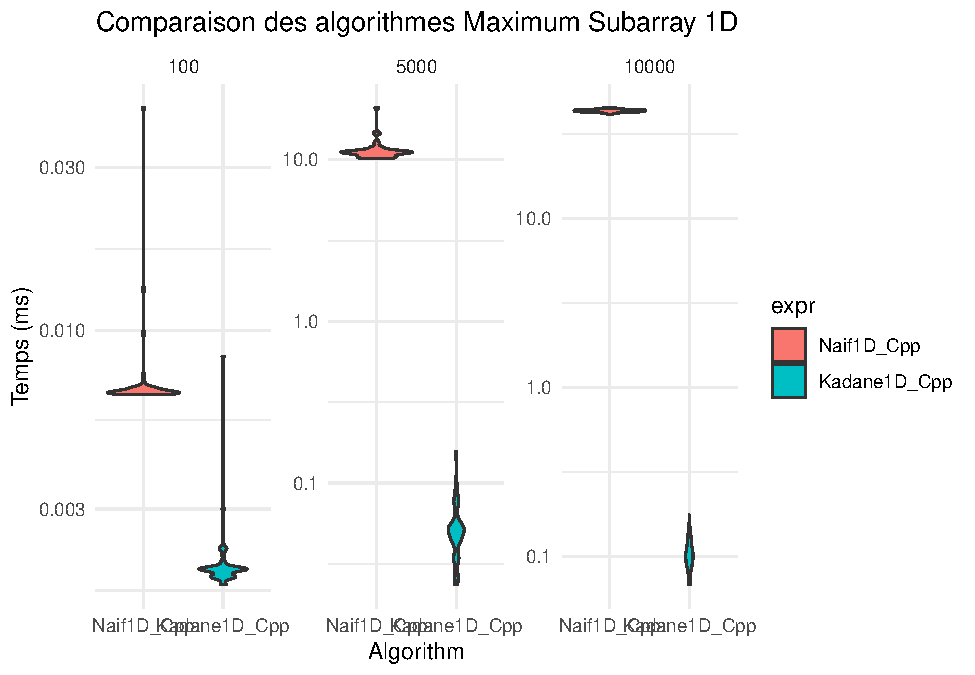
\includegraphics{MaxSubarray1D_files/figure-latex/benchmark-1.pdf}

\begin{verbatim}
## # A tibble: 6 x 8
##       n expr         min_time q1_time median_time mean_time q3_time max_time
##   <dbl> <fct>           <dbl>   <dbl>       <dbl>     <dbl>   <dbl>    <dbl>
## 1   100 Naif1D_Cpp     0.0041  0.0041      0.0042   0.00480  0.0043   0.0279
## 2   100 Kadane1D_Cpp   0.0011  0.0012      0.0012   0.00137  0.0013   0.007 
## 3  5000 Naif1D_Cpp     6.37    6.61        6.88     7.05     7.22     9.80  
## 4  5000 Kadane1D_Cpp   0.0174  0.0282      0.0314   0.0330   0.0350   0.0868
## 5 10000 Naif1D_Cpp    26.0    27.3        28.0     28.9     29.7     39.2   
## 6 10000 Kadane1D_Cpp   0.0446  0.0563      0.0656   0.0691   0.0729   0.198
\end{verbatim}

\begin{center}\rule{0.5\linewidth}{0.5pt}\end{center}

\section{Evaluation de la
complexité}\label{evaluation-de-la-complexituxe9}

Les vecteurs de longueurs \texttt{vector\_n\_naive} et
\texttt{vector\_n\_kadane} (\texttt{n} dans les dataframes) sont choisis
sur l'echelle logarithmique afin d'avoir un pas constant sur l'échelle
logarithmique en abscisse pour la régression.

On réalise 10 répétitions pour chaque valeur de \texttt{n} et pour
chaque algorithme. Les barres d'erreur sont placées en ``mean +/- sd''.

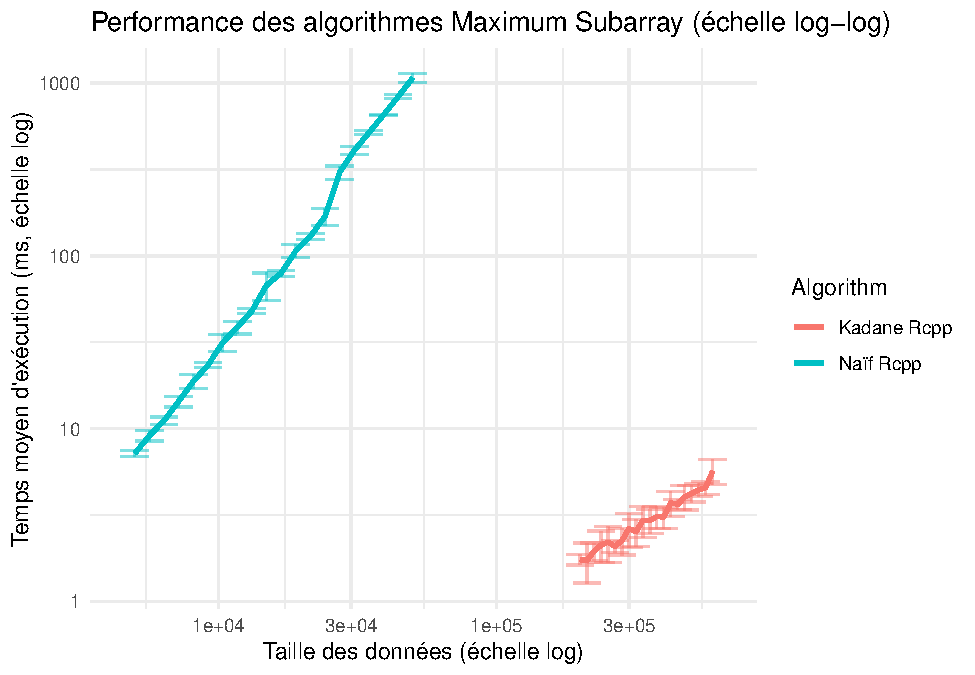
\includegraphics{MaxSubarray1D_files/figure-latex/simu complexite-1.pdf}

\begin{Shaded}
\begin{Highlighting}[]
\CommentTok{\# Affichage des résultats}
\FunctionTok{cat}\NormalTok{(}\StringTok{"Les résultats pour la solution naïve:}\SpecialCharTok{\textbackslash{}n}\StringTok{"}\NormalTok{)}
\end{Highlighting}
\end{Shaded}

\begin{verbatim}
## Les résultats pour la solution naïve:
\end{verbatim}

\begin{Shaded}
\begin{Highlighting}[]
\NormalTok{res\_Naive}
\end{Highlighting}
\end{Shaded}

\begin{verbatim}
##        n mean_time    sd_time
## 1   5000     7.200  0.2991841
## 2   5644     9.123  0.6236817
## 3   6371    11.145  0.5563622
## 4   7192    14.405  1.0457028
## 5   8119    18.808  1.7312603
## 6   9165    23.307  0.7777610
## 7  10346    31.505  3.4447424
## 8  11679    38.573  3.1766336
## 9  13183    47.995  1.7669072
## 10 14882    67.621 12.1391876
## 11 16799    79.465  3.1507398
## 12 18963   106.873  9.0534046
## 13 21407   129.639  5.6214538
## 14 24165   169.168 18.5884318
## 15 27278   304.334 26.6861459
## 16 30792   406.982 21.8300582
## 17 34760   514.950 13.7058917
## 18 39238   653.446  7.1864088
## 19 44293   832.811 21.2956383
## 20 50000  1070.974 60.7800569
\end{verbatim}

\begin{Shaded}
\begin{Highlighting}[]
\FunctionTok{cat}\NormalTok{(}\StringTok{"Les résultats pour la solution optimale:}\SpecialCharTok{\textbackslash{}n}\StringTok{"}\NormalTok{)}
\end{Highlighting}
\end{Shaded}

\begin{verbatim}
## Les résultats pour la solution optimale:
\end{verbatim}

\begin{Shaded}
\begin{Highlighting}[]
\NormalTok{res\_Kadane}
\end{Highlighting}
\end{Shaded}

\begin{verbatim}
##         n mean_time   sd_time
## 1  200000     1.751 0.1177993
## 2  211905     1.734 0.4513240
## 3  224519     1.962 0.2241428
## 4  237884     2.128 0.4366489
## 5  252044     2.210 0.5221749
## 6  267047     2.091 0.1706491
## 7  282944     2.259 0.3977841
## 8  299786     2.651 0.6001009
## 9  317631     2.538 0.4588827
## 10 336539     2.956 0.5970520
## 11 356571     2.960 0.4703190
## 12 377797     3.111 0.4523875
## 13 400285     3.091 0.4317780
## 14 424113     3.724 0.6257476
## 15 449359     3.663 0.2389351
## 16 476107     4.037 0.6447403
## 17 504448     4.229 0.4569087
## 18 534476     4.429 0.3795158
## 19 566291     4.577 0.4072687
## 20 600000     5.682 0.9350793
\end{verbatim}

On vérifie la valeur du coefficient directeur pour les deux méthodes:

\begin{verbatim}
## 
## Call:
## lm(formula = log(res_Naive$mean_time) ~ log(res_Naive$n))
## 
## Residuals:
##      Min       1Q   Median       3Q      Max 
## -0.19432 -0.07602  0.02344  0.08923  0.14727 
## 
## Coefficients:
##                   Estimate Std. Error t value Pr(>|t|)    
## (Intercept)      -17.00864    0.34524  -49.27   <2e-16 ***
## log(res_Naive$n)   2.21288    0.03562   62.13   <2e-16 ***
## ---
## Signif. codes:  0 '***' 0.001 '**' 0.01 '*' 0.05 '.' 0.1 ' ' 1
## 
## Residual standard error: 0.1113 on 18 degrees of freedom
## Multiple R-squared:  0.9954, Adjusted R-squared:  0.9951 
## F-statistic:  3860 on 1 and 18 DF,  p-value: < 2.2e-16
\end{verbatim}

\begin{verbatim}
## Exposant estimé (naïf): 2.21288
\end{verbatim}

\begin{verbatim}
## 
## Call:
## lm(formula = log(res_Kadane$mean_time) ~ log(res_Kadane$n))
## 
## Residuals:
##       Min        1Q    Median        3Q       Max 
## -0.086471 -0.033685 -0.008933  0.039289  0.119393 
## 
## Coefficients:
##                    Estimate Std. Error t value Pr(>|t|)    
## (Intercept)       -11.62733    0.45467  -25.57 1.33e-15 ***
## log(res_Kadane$n)   0.99553    0.03563   27.94 2.81e-16 ***
## ---
## Signif. codes:  0 '***' 0.001 '**' 0.01 '*' 0.05 '.' 0.1 ' ' 1
## 
## Residual standard error: 0.05313 on 18 degrees of freedom
## Multiple R-squared:  0.9775, Adjusted R-squared:  0.9762 
## F-statistic: 780.6 on 1 and 18 DF,  p-value: 2.815e-16
\end{verbatim}

\begin{verbatim}
## Exposant estimé (Kadane): 0.9955319
\end{verbatim}

Les coefficients directeurs trouvés sont bien ceux que l'on attendait.
La valeur 2 pour la méthode naïve et 1 pour l'algorithme de Kadane

\begin{center}\rule{0.5\linewidth}{0.5pt}\end{center}

\section{Cas particulier des données presques
triées}\label{cas-particulier-des-donnuxe9es-presques-triuxe9es}

On considère des données triées avec 5\% de valeurs échangées au hasard.

Sur un exemple cela donne :

\begin{Shaded}
\begin{Highlighting}[]
\NormalTok{v }\OtherTok{\textless{}{-}} \DecValTok{1}\SpecialCharTok{:}\DecValTok{100}
\NormalTok{n\_swap }\OtherTok{\textless{}{-}} \FunctionTok{floor}\NormalTok{(}\FloatTok{0.05} \SpecialCharTok{*} \FunctionTok{length}\NormalTok{(v))}
\NormalTok{swap\_indices }\OtherTok{\textless{}{-}} \FunctionTok{sample}\NormalTok{(}\FunctionTok{length}\NormalTok{(v), n\_swap)}
\NormalTok{v[swap\_indices] }\OtherTok{\textless{}{-}} \FunctionTok{sample}\NormalTok{(v[swap\_indices])}
\NormalTok{v}
\end{Highlighting}
\end{Shaded}

\begin{verbatim}
##   [1]   1   2   3   4   5   6   7   8   9  10  11  12  13  14  15  16  59  18
##  [19]  19  20  21  22  23  24  25  26  27  28  29  30  31  32  33  34  35  36
##  [37]  37  38  39  40  41  42  43  44  45  46  47  48  49  50  51  52  53  54
##  [55]  55  56  57  58  17  60  61  62  63  64  65  66  67  68  69  70  71  72
##  [73]  73  74  75  76  77  78  79  80  81  82  83  84  87  86  85  88  89  90
##  [91]  91  92  93  94  95  96  97  98  99 100
\end{verbatim}

\begin{Shaded}
\begin{Highlighting}[]
\CommentTok{\# Fonctions de simulation}
\NormalTok{one.simu }\OtherTok{\textless{}{-}} \ControlFlowTok{function}\NormalTok{(n, func) \{}
\NormalTok{  v }\OtherTok{\textless{}{-}} \FunctionTok{sample}\NormalTok{(}\SpecialCharTok{{-}}\DecValTok{100}\SpecialCharTok{:}\DecValTok{100}\NormalTok{, n, }\AttributeTok{replace =} \ConstantTok{TRUE}\NormalTok{)}
  \ControlFlowTok{if}\NormalTok{ (func }\SpecialCharTok{==} \StringTok{"Naive1D\_cpp"}\NormalTok{) }\FunctionTok{return}\NormalTok{(}\FunctionTok{max\_subarray\_sum\_naive\_Rcpp}\NormalTok{(v))}
  \ControlFlowTok{if}\NormalTok{ (func }\SpecialCharTok{==} \StringTok{"Kadane1D\_cpp"}\NormalTok{) }\FunctionTok{return}\NormalTok{(}\FunctionTok{max\_subarray\_sum\_opt\_Rcpp}\NormalTok{(v))}
\NormalTok{\}}

\NormalTok{one.simu2 }\OtherTok{\textless{}{-}} \ControlFlowTok{function}\NormalTok{(n, func) \{}
\NormalTok{  v }\OtherTok{\textless{}{-}} \DecValTok{1}\SpecialCharTok{:}\NormalTok{n}
\NormalTok{  n\_swap }\OtherTok{\textless{}{-}} \FunctionTok{floor}\NormalTok{(}\FloatTok{0.05} \SpecialCharTok{*}\NormalTok{ n)}
\NormalTok{  swap\_indices }\OtherTok{\textless{}{-}} \FunctionTok{sample}\NormalTok{(n, n\_swap)}
\NormalTok{  v[swap\_indices] }\OtherTok{\textless{}{-}} \FunctionTok{sample}\NormalTok{(v[swap\_indices])}
  \ControlFlowTok{if}\NormalTok{ (func }\SpecialCharTok{==} \StringTok{"Naive1D\_cpp"}\NormalTok{) }\FunctionTok{return}\NormalTok{(}\FunctionTok{max\_subarray\_sum\_naive\_Rcpp}\NormalTok{(v))}
  \ControlFlowTok{if}\NormalTok{ (func }\SpecialCharTok{==} \StringTok{"Kadane1D\_cpp"}\NormalTok{) }\FunctionTok{return}\NormalTok{(}\FunctionTok{max\_subarray\_sum\_opt\_Rcpp}\NormalTok{(v))}
\NormalTok{\}}
\end{Highlighting}
\end{Shaded}

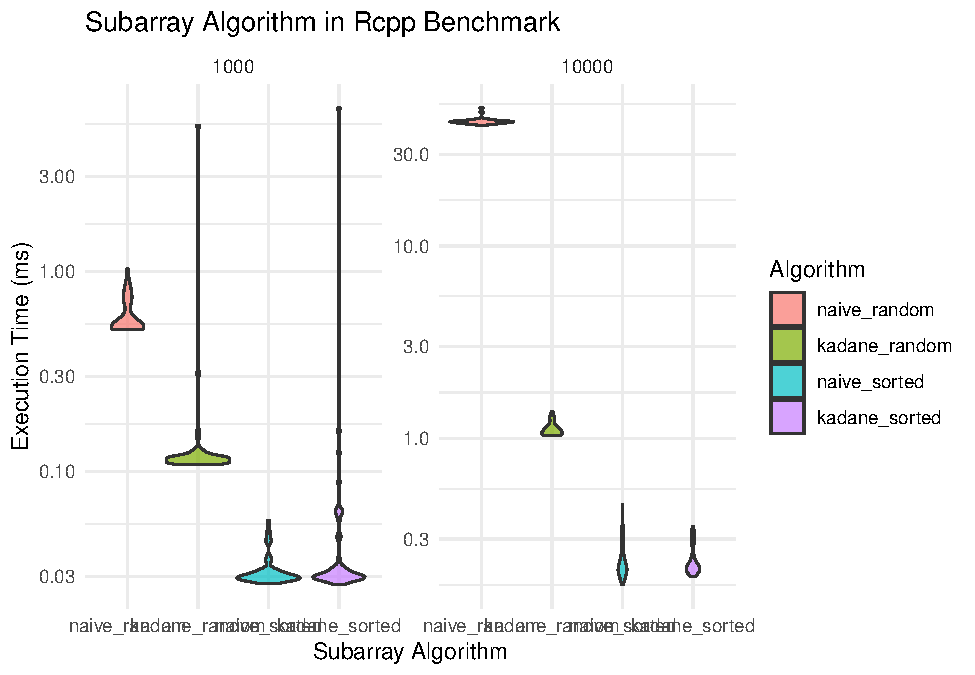
\includegraphics{MaxSubarray1D_files/figure-latex/benchmark2-1.pdf}

\begin{verbatim}
## # A tibble: 8 x 10
##       n expr       min_time q1_time median_time mean_time q3_time max_time type 
##   <dbl> <fct>         <dbl>   <dbl>       <dbl>     <dbl>   <dbl>    <dbl> <chr>
## 1  1000 naive_ran~   0.328   0.524       0.551     0.673   0.589    5.73   rand~
## 2  1000 kadane_ra~   0.0699  0.111       0.113     0.117   0.123    0.232  rand~
## 3  1000 naive_sor~   0.0182  0.0291      0.0312    0.0346  0.0346   0.0701 sort~
## 4  1000 kadane_so~   0.0194  0.0286      0.0306    0.168   0.0346   6.71   sort~
## 5 10000 naive_ran~  38.6    42.3        44.0      49.4    52.2     82.3    rand~
## 6 10000 kadane_ra~   0.677   1.01        1.12      1.13    1.28     1.67   rand~
## 7 10000 naive_sor~   0.122   0.215       0.246     0.292   0.301    1.77   sort~
## 8 10000 kadane_so~   0.139   0.212       0.241     0.249   0.286    0.398  sort~
## # i 1 more variable: algo <chr>
\end{verbatim}

Pour n = 1000, le temps d'exécution est plus rapide que pour n = 10000.
Kadane est toujours plus rapide que Naïf, avec un écart plus important à
n = 10000. Lorsque les tableaux sont triés, Naïf et Kadane sont beaucoup
plus rapides, avec un écart réduit entre les deux.

\section{Cas particulier des données presques toutes
positives}\label{cas-particulier-des-donnuxe9es-presques-toutes-positives}

On considère un vecteur contenant des valeurs positives, avec 5\% de
valeurs négatives insérées aléatoirement dans le vecteur.

Sur un exemple cela donne :

\begin{Shaded}
\begin{Highlighting}[]
\FunctionTok{set.seed}\NormalTok{(}\DecValTok{123}\NormalTok{)}

\CommentTok{\# Vecteur de base : valeurs positives de 1 à 100}
\NormalTok{v\_mostly\_pos }\OtherTok{\textless{}{-}} \FunctionTok{sample}\NormalTok{(}\DecValTok{1}\SpecialCharTok{:}\DecValTok{100}\NormalTok{)}

\CommentTok{\# Introduire 5\% de valeurs négatives aléatoires}
\NormalTok{n\_neg }\OtherTok{\textless{}{-}} \FunctionTok{floor}\NormalTok{(}\FloatTok{0.05} \SpecialCharTok{*} \FunctionTok{length}\NormalTok{(v\_mostly\_pos))  }\CommentTok{\# 5\% de négatifs}
\NormalTok{neg\_indices }\OtherTok{\textless{}{-}} \FunctionTok{sample}\NormalTok{(}\FunctionTok{length}\NormalTok{(v\_mostly\_pos), n\_neg)}

\CommentTok{\# Remplacer ces valeurs par des valeurs négatives aléatoires}
\NormalTok{v\_mostly\_pos[neg\_indices] }\OtherTok{\textless{}{-}} \SpecialCharTok{{-}}\FunctionTok{sample}\NormalTok{(}\DecValTok{1}\SpecialCharTok{:}\DecValTok{100}\NormalTok{, n\_neg)}

\CommentTok{\# Affichage du vecteur}
\NormalTok{v\_mostly\_pos}
\end{Highlighting}
\end{Shaded}

\begin{verbatim}
##   [1]  31  79  51  14  67  42  50  43  97  25  90  69  57   9  72  26 -94  95
##  [19]  87  36  78  93  76  15  32  84  82  41  23  27  60  53  75  89  71  38
##  [37]  91  34  29   5   8  12  13  18  33 -35  64  65  21  77  73  47  85 100
##  [55]  16  30   6  99  70  22  94 -79  49  17  63   4  58  61  40  96  19  54
##  [73]  20  80  62 -46  86   3  83  46  59  48  24 -54  81  68  88  98  44  10
##  [91]  56  11  55  37   2  28  74  35  52   1
\end{verbatim}

\begin{Shaded}
\begin{Highlighting}[]
\CommentTok{\# Fonctions de simulation}
\NormalTok{one.simu }\OtherTok{\textless{}{-}} \ControlFlowTok{function}\NormalTok{(n, func) \{}
\NormalTok{  v }\OtherTok{\textless{}{-}} \FunctionTok{sample}\NormalTok{(}\SpecialCharTok{{-}}\DecValTok{100}\SpecialCharTok{:}\DecValTok{100}\NormalTok{, n, }\AttributeTok{replace =} \ConstantTok{TRUE}\NormalTok{)}
  \ControlFlowTok{if}\NormalTok{ (func }\SpecialCharTok{==} \StringTok{"Naive1D\_cpp"}\NormalTok{) }\FunctionTok{return}\NormalTok{(}\FunctionTok{max\_subarray\_sum\_naive\_Rcpp}\NormalTok{(v))}
  \ControlFlowTok{if}\NormalTok{ (func }\SpecialCharTok{==} \StringTok{"Kadane1D\_cpp"}\NormalTok{) }\FunctionTok{return}\NormalTok{(}\FunctionTok{max\_subarray\_sum\_opt\_Rcpp}\NormalTok{(v))}
\NormalTok{\}}

\NormalTok{one.simu2 }\OtherTok{\textless{}{-}} \ControlFlowTok{function}\NormalTok{(n, func) \{}
\NormalTok{  v\_mostly\_pos }\OtherTok{\textless{}{-}} \FunctionTok{sample}\NormalTok{(}\DecValTok{1}\SpecialCharTok{:}\DecValTok{100}\NormalTok{)}
\NormalTok{  n\_neg }\OtherTok{\textless{}{-}} \FunctionTok{floor}\NormalTok{(}\FloatTok{0.05} \SpecialCharTok{*} \FunctionTok{length}\NormalTok{(v\_mostly\_pos))}
\NormalTok{  neg\_indices }\OtherTok{\textless{}{-}} \FunctionTok{sample}\NormalTok{(}\FunctionTok{length}\NormalTok{(v\_mostly\_pos), n\_neg)}
\NormalTok{  v\_mostly\_pos[neg\_indices] }\OtherTok{\textless{}{-}} \SpecialCharTok{{-}}\FunctionTok{sample}\NormalTok{(}\DecValTok{1}\SpecialCharTok{:}\DecValTok{100}\NormalTok{, n\_neg)}
  \ControlFlowTok{if}\NormalTok{ (func }\SpecialCharTok{==} \StringTok{"Naive1D\_cpp"}\NormalTok{) }\FunctionTok{return}\NormalTok{(}\FunctionTok{max\_subarray\_sum\_naive\_Rcpp}\NormalTok{(v\_mostly\_pos))}
  \ControlFlowTok{if}\NormalTok{ (func }\SpecialCharTok{==} \StringTok{"Kadane1D\_cpp"}\NormalTok{) }\FunctionTok{return}\NormalTok{(}\FunctionTok{max\_subarray\_sum\_opt\_Rcpp}\NormalTok{(v\_mostly\_pos))}
\NormalTok{\}}
\end{Highlighting}
\end{Shaded}

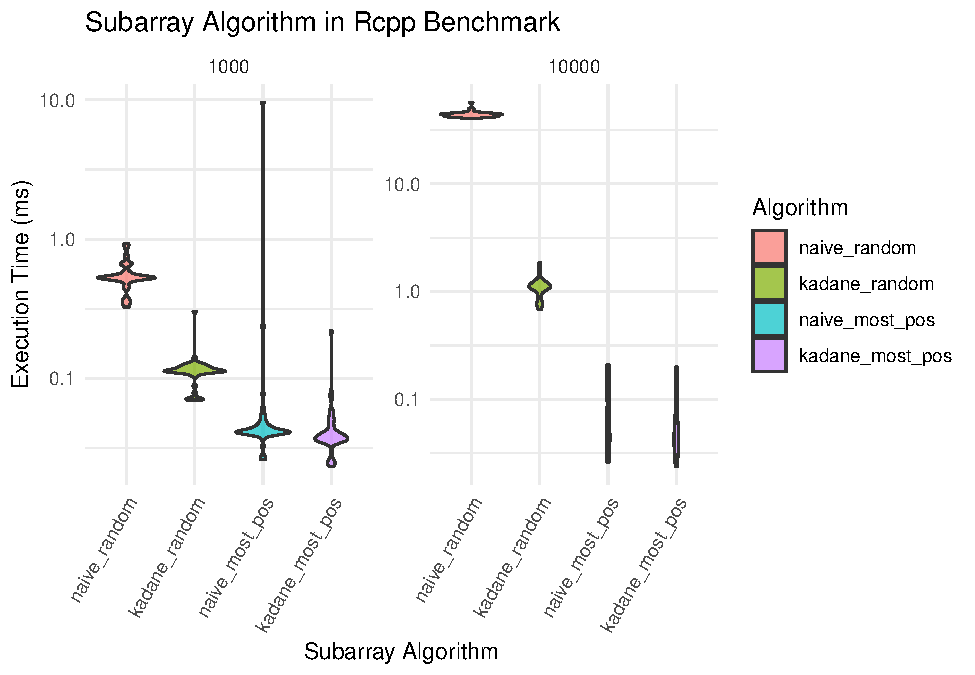
\includegraphics{MaxSubarray1D_files/figure-latex/benchmark3-1.pdf}

\section{Cas particulier des données presques toutes
negatives}\label{cas-particulier-des-donnuxe9es-presques-toutes-negatives}

On considère un vecteur contenant des valeurs négatives, avec 5\% de
valeurs positives insérées aléatoirement dans le vecteur.

Sur un exemple cela donne :

\begin{Shaded}
\begin{Highlighting}[]
\FunctionTok{set.seed}\NormalTok{(}\DecValTok{123}\NormalTok{)}

\CommentTok{\# Vecteur de base : valeurs négatives de {-}1 à {-}100}
\NormalTok{v\_mostly\_neg }\OtherTok{\textless{}{-}} \SpecialCharTok{{-}}\FunctionTok{sample}\NormalTok{(}\DecValTok{1}\SpecialCharTok{:}\DecValTok{100}\NormalTok{)}

\CommentTok{\# Introduire 5\% de valeurs positives aléatoires}
\NormalTok{n\_pos }\OtherTok{\textless{}{-}} \FunctionTok{floor}\NormalTok{(}\FloatTok{0.05} \SpecialCharTok{*} \FunctionTok{length}\NormalTok{(v\_mostly\_neg))  }\CommentTok{\# 5\% de positifs}
\NormalTok{pos\_indices }\OtherTok{\textless{}{-}} \FunctionTok{sample}\NormalTok{(}\FunctionTok{length}\NormalTok{(v\_mostly\_neg), n\_pos)}

\CommentTok{\# Remplacer ces valeurs par des valeurs positives aléatoires}
\NormalTok{v\_mostly\_neg[pos\_indices] }\OtherTok{\textless{}{-}} \FunctionTok{sample}\NormalTok{(}\DecValTok{1}\SpecialCharTok{:}\DecValTok{100}\NormalTok{, n\_pos)}

\CommentTok{\# Affichage du vecteur}
\NormalTok{v\_mostly\_neg}
\end{Highlighting}
\end{Shaded}

\begin{verbatim}
##   [1]  -31  -79  -51  -14  -67  -42  -50  -43  -97  -25  -90  -69  -57   -9  -72
##  [16]  -26   94  -95  -87  -36  -78  -93  -76  -15  -32  -84  -82  -41  -23  -27
##  [31]  -60  -53  -75  -89  -71  -38  -91  -34  -29   -5   -8  -12  -13  -18  -33
##  [46]   35  -64  -65  -21  -77  -73  -47  -85 -100  -16  -30   -6  -99  -70  -22
##  [61]  -94   79  -49  -17  -63   -4  -58  -61  -40  -96  -19  -54  -20  -80  -62
##  [76]   46  -86   -3  -83  -46  -59  -48  -24   54  -81  -68  -88  -98  -44  -10
##  [91]  -56  -11  -55  -37   -2  -28  -74  -35  -52   -1
\end{verbatim}

\begin{Shaded}
\begin{Highlighting}[]
\CommentTok{\# Fonctions de simulation}
\NormalTok{one.simu }\OtherTok{\textless{}{-}} \ControlFlowTok{function}\NormalTok{(n, func) \{}
\NormalTok{  v }\OtherTok{\textless{}{-}} \FunctionTok{sample}\NormalTok{(}\SpecialCharTok{{-}}\DecValTok{100}\SpecialCharTok{:}\DecValTok{100}\NormalTok{, n, }\AttributeTok{replace =} \ConstantTok{TRUE}\NormalTok{)}
  \ControlFlowTok{if}\NormalTok{ (func }\SpecialCharTok{==} \StringTok{"Naive1D\_cpp"}\NormalTok{) }\FunctionTok{return}\NormalTok{(}\FunctionTok{max\_subarray\_sum\_naive\_Rcpp}\NormalTok{(v))}
  \ControlFlowTok{if}\NormalTok{ (func }\SpecialCharTok{==} \StringTok{"Kadane1D\_cpp"}\NormalTok{) }\FunctionTok{return}\NormalTok{(}\FunctionTok{max\_subarray\_sum\_opt\_Rcpp}\NormalTok{(v))}
\NormalTok{\}}

\NormalTok{one.simu2 }\OtherTok{\textless{}{-}} \ControlFlowTok{function}\NormalTok{(n, func) \{}

\NormalTok{  v\_mostly\_neg }\OtherTok{\textless{}{-}} \SpecialCharTok{{-}}\FunctionTok{sample}\NormalTok{(}\DecValTok{1}\SpecialCharTok{:}\DecValTok{100}\NormalTok{)}
\NormalTok{  n\_pos }\OtherTok{\textless{}{-}} \FunctionTok{floor}\NormalTok{(}\FloatTok{0.05} \SpecialCharTok{*} \FunctionTok{length}\NormalTok{(v\_mostly\_neg))}
\NormalTok{  pos\_indices }\OtherTok{\textless{}{-}} \FunctionTok{sample}\NormalTok{(}\FunctionTok{length}\NormalTok{(v\_mostly\_neg), n\_pos)}
\NormalTok{  v\_mostly\_neg[pos\_indices] }\OtherTok{\textless{}{-}} \FunctionTok{sample}\NormalTok{(}\DecValTok{1}\SpecialCharTok{:}\DecValTok{100}\NormalTok{, n\_pos)}
  \ControlFlowTok{if}\NormalTok{ (func }\SpecialCharTok{==} \StringTok{"Naive1D\_cpp"}\NormalTok{) }\FunctionTok{return}\NormalTok{(}\FunctionTok{max\_subarray\_sum\_naive\_Rcpp}\NormalTok{(v\_mostly\_neg ))}
  \ControlFlowTok{if}\NormalTok{ (func }\SpecialCharTok{==} \StringTok{"Kadane1D\_cpp"}\NormalTok{) }\FunctionTok{return}\NormalTok{(}\FunctionTok{max\_subarray\_sum\_opt\_Rcpp}\NormalTok{(v\_mostly\_neg ))}
\NormalTok{\}}
\end{Highlighting}
\end{Shaded}

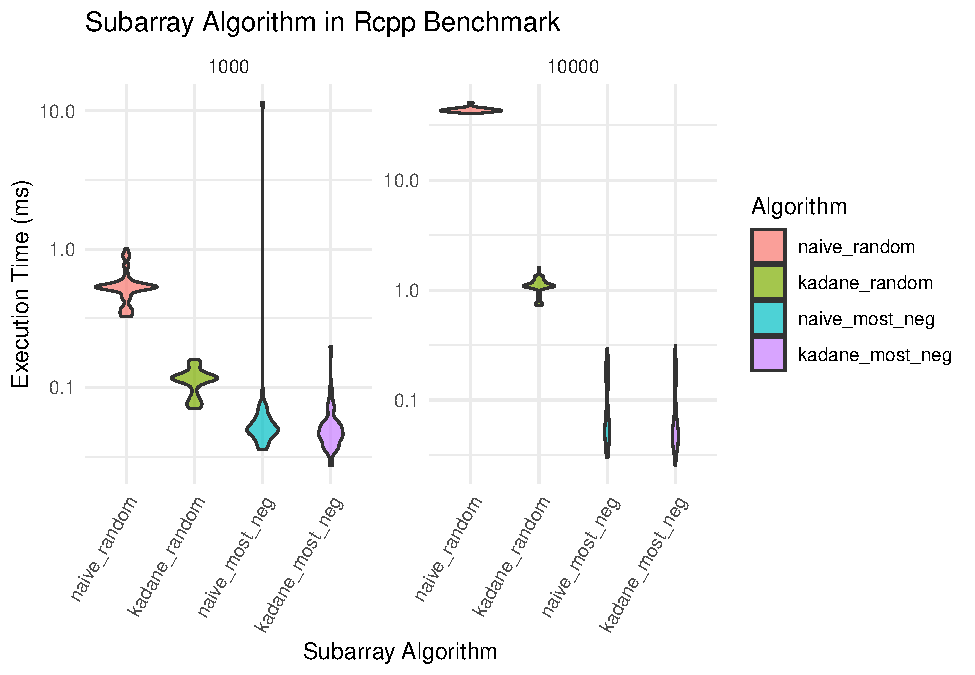
\includegraphics{MaxSubarray1D_files/figure-latex/benchmark4-1.pdf}

\begin{verbatim}
## # A tibble: 8 x 10
##       n expr       min_time q1_time median_time mean_time q3_time max_time type 
##   <dbl> <fct>         <dbl>   <dbl>       <dbl>     <dbl>   <dbl>    <dbl> <chr>
## 1  1000 naive_ran~   0.327   0.476       0.530     0.541   0.553     1.00  rand~
## 2  1000 kadane_ra~   0.0708  0.0990      0.116     0.112   0.120     0.159 rand~
## 3  1000 naive_mos~   0.0355  0.0464      0.0498    0.282   0.0588   11.5   rand~
## 4  1000 kadane_mo~   0.0273  0.0419      0.0464    0.0532  0.0544    0.198 rand~
## 5 10000 naive_ran~  40.3    42.3        43.4      43.7    44.6      51.3   rand~
## 6 10000 kadane_ra~   0.724   1.06        1.09      1.09    1.19      1.61  rand~
## 7 10000 naive_mos~   0.0299  0.0476      0.0586    0.0983  0.169     0.292 rand~
## 8 10000 kadane_mo~   0.0253  0.0426      0.0523    0.0821  0.0822    0.311 rand~
## # i 1 more variable: algo <chr>
\end{verbatim}

Pour n = 1000, le temps d'exécution est plus rapide que pour n = 10000.
Kadane est toujours plus rapide que Naïf, avec un écart plus important à
n = 10000. Lorsque les tableaux sont presques toutes négatif, Naïf et
Kadane sont beaucoup plus rapides, avec un écart réduit entre les deux.

\end{document}
